% ============================================================
%  CHAPTER 8: GRAVITATION
%  The Physics Codex: A Complete University Foundation
%  Korede Samuel Omotosho (Falcon)
%  Aurikrex Learning Systems, 2026
%
%  File: chapters/part1/ch08_gravitation.tex
% ============================================================

\chapter{Gravitation}
\label{ch:gravitation}

\chapterquote{Gravity explains the motions of the planets,
but it cannot explain who set the planets in motion.}{Isaac Newton}

\begin{objectivebox}
By the end of this chapter, you should be able to:
\begin{enumerate}[noitemsep]
  \item State Newton's Law of Universal Gravitation
  and apply it to calculate gravitational forces
  \item Define gravitational field strength and
  calculate it at various distances from a mass
  \item Derive the relationship between $g$ at the
  surface and at height $h$ above the surface
  \item Define gravitational potential energy and
  gravitational potential
  \item Derive and apply escape velocity
  \item Explain satellite motion and derive orbital
  speed and period
  \item State Kepler's three laws and verify them
  mathematically
  \item Explain weightlessness in orbit
\end{enumerate}
\end{objectivebox}

\vspace{0.5cm}

% ============================================================
\section{The Universal Nature of Gravity}
% ============================================================

Before Newton, gravity was thought of as a purely
terrestrial phenomenon --- the reason things fall
down on Earth. The planets, it was assumed, were kept
in their orbits by some entirely separate celestial
mechanism. Newton's greatest insight was recognising
that these were the same force.

The Moon, Newton reasoned, is $60$ Earth radii away.
If gravity follows an inverse square law, then the
gravitational acceleration at the Moon should be:
\[
  g_{Moon} = \frac{g_{surface}}{60^2}
  = \frac{9.81}{3600} \approx 0.00272\ \text{m\,s}^{-2}
\]
The Moon's centripetal acceleration in its orbit
(calculated from its orbital speed and radius) is
$0.00272\ \text{m\,s}^{-2}$.

The match was exact. The same force that drops an
apple holds the Moon in its orbit. This was one of
the most profound unifications in the history of
science.

% ============================================================
\section{Newton's Law of Universal Gravitation}
% ============================================================

\begin{lawbox}[Newton's Law of Universal Gravitation]
Every particle of matter in the universe attracts
every other particle with a force that is:
\begin{itemize}[noitemsep]
  \item Directly proportional to the product of
  their masses
  \item Inversely proportional to the square of the
  distance between them
  \item Directed along the line joining them
\end{itemize}
\[
  F = \frac{Gm_1 m_2}{r^2}
\]
where $G = 6.674 \times 10^{-11}\ \text{N\,m}^2\text{kg}^{-2}$
is the \textbf{universal gravitational constant}.
\end{lawbox}

\begin{diagbox}[Gravitational Force Between Two Masses]
\begin{center}
\begin{tikzpicture}[scale=1.0]
  % Masses
  \fill[codexblue!60] (-3,0) circle (0.4cm)
    node[below=0.5cm]{$m_1$};
  \fill[codexred!60] (3,0) circle (0.5cm)
    node[below=0.6cm]{$m_2$};

  % Force arrows
  \draw[->, very thick, codexblue]
    (-2.5,0) -- (-1.2,0)
    node[above, font=\small]{$F$ on $m_1$};
  \draw[->, very thick, codexred]
    (2.5,0) -- (1.2,0)
    node[above, font=\small]{$F$ on $m_2$};

  % Distance
  \draw[<->, gray, thick] (-3,-1) -- (3,-1);
  \node[below, gray] at (0,-1) {$r$};

  % Equal and opposite annotation
  \node[font=\small, align=center] at (0,1.2)
    {Equal magnitudes, opposite directions\\
    (Newton's Third Law)};
\end{tikzpicture}
\end{center}
\end{diagbox}

\begin{historybox}[Measuring G: The Cavendish Experiment]
Newton could formulate the law but could not measure
$G$ directly --- the gravitational force between
laboratory-sized masses is extraordinarily small.
In 1798, Henry Cavendish used a delicate torsion balance:
two small lead balls on a horizontal rod suspended by
a thin fibre. Two large lead balls brought near the
small ones twisted the fibre measurably. From the
twist angle, Cavendish calculated $G$ with remarkable
accuracy. His experiment also allowed him to calculate
the mass (and hence density) of the Earth --- which is
why the Cavendish experiment is sometimes called
``weighing the Earth.''
\end{historybox}

\begin{examplebox}[8.1]
\stepcounter{workedexample}
Calculate the gravitational force between:
(a) two $70\ \text{kg}$ people standing $1.0\ \text{m}$
apart;
(b) the Earth and the Moon.\\
($M_E = 5.97\times10^{24}\ \text{kg}$,
$M_M = 7.35\times10^{22}\ \text{kg}$,
$r_{EM} = 3.84\times10^8\ \text{m}$,
$G = 6.67\times10^{-11}\ \text{N\,m}^2\text{kg}^{-2}$)
\end{examplebox}

\begin{solutionbox}
\textbf{(a)} Between two people:
\[
  F = \frac{Gm_1m_2}{r^2}
  = \frac{6.67\times10^{-11} \times 70 \times 70}{1.0^2}
  = \frac{6.67\times10^{-11} \times 4900}{1}
  = 3.27\times10^{-7}\ \text{N}
\]
This is about $0.33\ \mu\text{N}$ --- completely
imperceptible. This is why we do not feel gravitational
attraction to the people around us.

\textbf{(b)} Earth-Moon:
\[
  F = \frac{6.67\times10^{-11}
    \times 5.97\times10^{24}
    \times 7.35\times10^{22}}
    {(3.84\times10^8)^2}
\]
\[
  = \frac{6.67\times10^{-11}
    \times 4.388\times10^{47}}
    {1.475\times10^{17}}
\]
\[
  = \frac{2.927\times10^{37}}{1.475\times10^{17}}
  = 1.98\times10^{20}\ \text{N}
\]

\begin{realworldbox}[The Moon and Nigeria's Tides]
This $1.98\times10^{20}\ \text{N}$ force between
Earth and Moon drives the ocean tides. Coastal Nigerian
cities --- Lagos, Port Harcourt, Calabar --- experience
tidal variations directly caused by this gravitational
force. Fishermen along the Bight of Benin have
understood tidal patterns for centuries, using them to
navigate. The physics behind those patterns is
Newton's equation above.
\end{realworldbox}
\end{solutionbox}

% ============================================================
\section{Gravitational Field Strength}
% ============================================================

\begin{definitionbox}[Gravitational Field]
A \textbf{gravitational field} exists in the space
around any mass. It is a region where another mass
experiences a gravitational force.

The \textbf{gravitational field strength} $g$ at a
point is the gravitational force per unit mass at
that point:
\[
  g = \frac{F}{m} = \frac{GM}{r^2}
\]
SI unit: N\,kg$^{-1}$ = m\,s$^{-2}$

At Earth's surface ($r = R_E$):
\[
  g_s = \frac{GM_E}{R_E^2}
  \approx 9.81\ \text{m\,s}^{-2}
\]
\end{definitionbox}

\subsection{Variation of \texorpdfstring{$g$}{g} with Height}

At height $h$ above Earth's surface, the distance
from the centre is $r = R_E + h$:
\[
  g_h = \frac{GM_E}{(R_E+h)^2}
\]

The ratio of $g$ at height $h$ to $g$ at the surface:
\[
  \frac{g_h}{g_s} = \frac{R_E^2}{(R_E+h)^2}
  = \left(\frac{R_E}{R_E+h}\right)^2
\]

\begin{examplebox}[8.2]
\stepcounter{workedexample}
The International Space Station orbits at
$h = 400\ \text{km}$ above Earth's surface.\\
(a) Calculate $g$ at that altitude.\\
(b) If $g$ is not zero there, why do astronauts
feel weightless?\\
($R_E = 6.4\times10^6\ \text{m}$,
$g_s = 9.81\ \text{m\,s}^{-2}$)
\end{examplebox}

\begin{solutionbox}
\textbf{(a)} $r = R_E + h
= 6.4\times10^6 + 4\times10^5
= 6.8\times10^6\ \text{m}$

\[
  g_h = g_s\left(\frac{R_E}{r}\right)^2
  = 9.81 \times \left(\frac{6.4\times10^6}
  {6.8\times10^6}\right)^2
  = 9.81 \times (0.9412)^2
  = 9.81 \times 0.885
  = 8.68\ \text{m\,s}^{-2}
\]

$g$ at the ISS altitude is about $88.5\%$ of its
surface value --- far from zero.

\textbf{(b)} The astronauts feel weightless because
they are in \textbf{free fall}. Both the astronauts
and the space station are falling toward Earth at
exactly the same rate --- the station's orbital
speed means it keeps missing the Earth. There is no
contact force (normal force) between the astronaut
and the floor, so they feel no weight. This is
called \textbf{apparent weightlessness}.
\end{solutionbox}

\subsection{Variation of \texorpdfstring{$g$}{g} with Depth}

Inside the Earth (at depth $d$ below the surface),
assuming uniform density:
\[
  g_d = g_s\left(1 - \frac{d}{R_E}\right)
  = g_s\frac{(R_E - d)}{R_E}
\]
$g$ decreases linearly with depth and equals zero
at the centre.

\begin{diagbox}[$g$ vs Distance from Earth's Centre]
\begin{center}
\begin{tikzpicture}
\begin{axis}[
  width=11cm, height=6cm,
  xlabel={Distance from centre ($\times 10^6$ m)},
  ylabel={Gravitational field strength $g$ (m\,s$^{-2}$)},
  xmin=0, xmax=20,
  ymin=0, ymax=12,
  grid=major, grid style={gray!20},
  xtick={0,2,4,6,8,10,12,14,16,18,20},
]
  % Inside Earth (linear, 0 to R_E = 6.4)
  \addplot[codexblue, very thick, domain=0:6.4, samples=50]{9.81*x/6.4};

  % Outside Earth (inverse square, R_E to 20)
  \addplot[codexred, very thick, domain=6.4:20, samples=100]{9.81*(6.4/x)^2};

  % Surface marker
  \draw[dashed, codexgold, thick] (axis cs:6.4,0) -- (axis cs:6.4,9.81);
  \node[codexgold, above, font=\small] at (axis cs:6.4,9.81)
    {\shortstack{Surface\\$g = 9.81$}};

  % Labels
  \node[codexblue, font=\small] at (axis cs:3,6) {\shortstack{Inside Earth\\(linear)}};
  \node[codexred, font=\small] at (axis cs:13,4)
    {\shortstack{Outside Earth\\(inverse square)}};
\end{axis}
\end{tikzpicture}
\end{center}

\vspace{0.4em}
{\small\itshape Assumption: Earth is modelled as a uniform-density sphere 
for this course. See the Real World box below for the actual behaviour.}
\end{diagbox}

\begin{realworldbox}{Earth's Actual Gravitational Profile}
The graph above assumes Earth has \textbf{uniform density} throughout. 
In reality, Earth's density increases significantly toward the core 
($\rho_{\text{core}} \approx 13{,}000\ \text{kg\,m}^{-3}$ vs 
$\rho_{\text{crust}} \approx 2{,}700\ \text{kg\,m}^{-3}$). 

This means the real $g$ actually \textit{increases slightly below the 
surface}, peaking near the core--mantle boundary at approximately 
$10.7\ \text{ms}^{-2}$, before falling to zero at the centre. 
The uniform-density model is the standard approximation used at 
this level.
\end{realworldbox}

% ============================================================
\section{Gravitational Potential Energy}
% ============================================================
 
\begin{definitionbox}[Gravitational Potential Energy]
The \textbf{gravitational potential energy} of a mass
$m$ at distance $r$ from the centre of mass $M$ is:
\[
  E_p = -\frac{GMm}{r}
\]
The negative sign indicates that gravity is an
\textit{attractive} force --- work must be done
\textit{against} gravity to move $m$ away from $M$.
$E_p = 0$ at $r = \infty$ (reference point).
 
For heights near Earth's surface where $h \ll R_E$,
this reduces to the familiar:
\[
  \Delta E_p = mgh
\]
\end{definitionbox}
 
\begin{definitionbox}[Gravitational Potential]
The \textbf{gravitational potential} $V$ at a point
is the work done per unit mass to move a test mass
from infinity to that point:
\[
  V = \frac{E_p}{m} = -\frac{GM}{r}
\]
SI unit: J\,kg$^{-1}$. Always negative (for attractive
field).
\end{definitionbox}
 
% ============================================================
\section{Escape Velocity}
% ============================================================
 
\begin{definitionbox}[Escape Velocity]
The \textbf{escape velocity} is the minimum speed
required for an object to escape from a gravitational
field to infinity (with zero kinetic energy at
$r = \infty$).
\end{definitionbox}
 
\begin{processbox}[Deriving Escape Velocity]
For a mass $m$ to escape from the surface of a planet
of mass $M$ and radius $R$:
 
Total energy at surface = Total energy at infinity:
\[
  \frac{1}{2}mv_{esc}^2 - \frac{GMm}{R}
  = 0 + 0
\]
\[
  \frac{1}{2}v_{esc}^2 = \frac{GM}{R}
\]
\[
  \boxed{v_{esc} = \sqrt{\frac{2GM}{R}} = \sqrt{2gR}}
\]
\end{processbox}
 
\begin{examplebox}[8.3]
\stepcounter{workedexample}
Calculate the escape velocity from:
(a) Earth's surface;
(b) the Moon's surface.\\
($M_E = 5.97\times10^{24}\ \text{kg}$,
$R_E = 6.4\times10^6\ \text{m}$,
$M_M = 7.35\times10^{22}\ \text{kg}$,
$R_M = 1.74\times10^6\ \text{m}$,
$G = 6.67\times10^{-11}\ \text{N\,m}^2\text{kg}^{-2}$)
\end{examplebox}
 
\begin{solutionbox}
\textbf{(a)} Earth:
\[
  v_{esc} = \sqrt{\frac{2GM_E}{R_E}}
  = \sqrt{\frac{2 \times 6.67\times10^{-11}
    \times 5.97\times10^{24}}{6.4\times10^6}}
\]
\[
   v_{esc} = \sqrt{\frac{7.96\times10^{14}}{6.4\times10^6}}
  = \sqrt{1.24\times10^8}
  = 11\,200\ \text{m\,s}^{-1} = 11.2\ \text{km\,s}^{-1}
\]
 
\textbf{(b)} Moon:
\[
  v_{esc} = \sqrt{\frac{2 \times 6.67\times10^{-11}
    \times 7.35\times10^{22}}{1.74\times10^6}}
  = \sqrt{\frac{9.80\times10^{12}}{1.74\times10^6}}
\]
\[
  v_{esc} = \sqrt{5.63\times10^6}
  = 2370\ \text{m\,s}^{-1} = 2.37\ \text{km\,s}^{-1}
\]
 
The Moon's escape velocity is only about $21\%$ of
Earth's. This is why the Moon has no atmosphere ---
gas molecules moving at typical thermal speeds can
escape the Moon's weak gravity entirely.
\end{solutionbox}
 
% ============================================================
\section{Kepler's Laws of Planetary Motion}
% ============================================================
 
Johannes Kepler (1571--1630) spent years analysing
the meticulous astronomical observations of Tycho
Brahe and extracted three empirical laws that
described planetary motion perfectly --- all before
Newton was born, and without any understanding of
\textit{why} they were true. Newton later showed
that all three follow mathematically from his Law
of Universal Gravitation.
 
\begin{lawbox}[Kepler's Three Laws]
\textbf{First Law (Law of Ellipses):}
Every planet moves in an elliptical orbit with the
Sun at one focus.
 
\vspace{0.5cm}
 
\textbf{Second Law (Law of Equal Areas):}
A line joining a planet to the Sun sweeps out equal
areas in equal time intervals. (Consequence: a planet
moves fastest when closest to the Sun --- perihelion
--- and slowest when furthest --- aphelion.)
 
\vspace{0.5cm}
 
\textbf{Third Law (Harmonic Law):}
The square of the orbital period is proportional to
the cube of the semi-major axis (mean orbital radius):
\[
  T^2 \propto r^3
  \quad \text{or} \quad
  \frac{T^2}{r^3} = \frac{4\pi^2}{GM}
  = \text{constant (for all planets around same star)}
\]
\end{lawbox}
 
\begin{processbox}[Deriving Kepler's Third Law from
Newton's Law]
For a circular orbit of radius $r$, the gravitational
force provides centripetal force:
\[
  \frac{GMm}{r^2} = \frac{mv^2}{r}
  = \frac{m(2\pi r/T)^2}{r}
  = \frac{4\pi^2 mr}{T^2}
\]
Rearranging:
\[
  T^2 = \frac{4\pi^2 r^3}{GM}
\]
Since $G$, $M$ (mass of Sun) are constant for all
planets in the solar system, $T^2/r^3$ is constant ---
exactly Kepler's Third Law.
\end{processbox}
 
\begin{examplebox}[8.4]
\stepcounter{workedexample}
Mars orbits the Sun at a mean distance of
$1.52\ \text{AU}$ (astronomical units), where
$1\ \text{AU} = 1.496\times10^{11}\ \text{m}$ is
Earth's mean orbital radius.
Earth's orbital period is $365.25$ days.
Calculate the orbital period of Mars.
\end{examplebox}
 
\begin{solutionbox}
Using Kepler's Third Law:
\[
  \frac{T_{Mars}^2}{T_{Earth}^2}
  = \frac{r_{Mars}^3}{r_{Earth}^3}
  = \left(\frac{r_{Mars}}{r_{Earth}}\right)^3
  = (1.52)^3 = 3.512
\]
\[
  T_{Mars}^2 = 3.512 \times T_{Earth}^2
  = 3.512 \times (365.25)^2
  = 3.512 \times 133\,408
  = 468\,530
\]
\[
  T_{Mars} = \sqrt{468\,530}
  = 684.5\ \text{days} \approx 687\ \text{days}
\]
The actual Martian year is $686.97$ days.
Our calculation gives excellent agreement.
\end{solutionbox}
 
% ============================================================
\section{Geostationary and Polar Satellites}
% ============================================================
 
\begin{definitionbox}[Types of Satellites]
\textbf{Geostationary satellite:}
Orbits above the equator with period $= 24$ hours
(same as Earth's rotation). Appears stationary
relative to the ground. Used for TV broadcasting,
weather monitoring, communications.
Orbital radius $\approx 42\,300\ \text{km}$ from
Earth's centre.
 
\vspace{0.4cm}
 
\textbf{Low Earth Orbit (LEO) satellite:}
Orbits at $200$--$2000\ \text{km}$ altitude.
Period $\approx 90$--$120$ minutes. Used for GPS,
imaging, the ISS.
 
\vspace{0.4cm}
 
\textbf{Polar orbit satellite:}
Passes over both poles. As Earth rotates beneath it,
the satellite can eventually scan the entire surface.
Used for Earth observation, weather satellites.
\end{definitionbox}
 
\begin{examplebox}[8.5]
\stepcounter{workedexample}
Calculate the orbital radius and orbital speed of a
geostationary satellite.
($M_E = 5.97\times10^{24}\ \text{kg}$,
$G = 6.67\times10^{-11}\ \text{N\,m}^2\text{kg}^{-2}$)
\end{examplebox}
 
\begin{solutionbox}
Period: $T = 24 \times 3600 = 86\,400\ \text{s}$
 
From $T^2 = 4\pi^2 r^3 / GM$:
\[
  r^3 = \frac{GM T^2}{4\pi^2}
  = \frac{6.67\times10^{-11}
    \times 5.97\times10^{24}
    \times (86400)^2}
    {4\pi^2}
\]
\[
  = \frac{6.67\times10^{-11}
    \times 5.97\times10^{24}
    \times 7.465\times10^9}
    {39.48}
\]
\[
  = \frac{2.976\times10^{24}}{39.48}
  = 7.539\times10^{22}\ \text{m}^3
\]
\[
  r = (7.539\times10^{22})^{1/3}
  = 4.22\times10^7\ \text{m}
  = 42\,200\ \text{km}
\]
 
Orbital speed:
\[
  v = \frac{2\pi r}{T}
  = \frac{2\pi \times 4.22\times10^7}{86400}
  = \frac{2.65\times10^8}{86400}
  = 3070\ \text{m\,s}^{-1}
  \approx 3.07\ \text{km\,s}^{-1}
\]
\end{solutionbox}

% ============================================================
\section{Chapter Summary}
% ============================================================

\begin{summarybox}
\textbf{Newton's Law of Gravitation:}
$F = GMm/r^2$; $G = 6.67\times10^{-11}\ \text{N\,m}^2\text{kg}^{-2}$

\textbf{Gravitational field strength:}
$g = GM/r^2$; at surface $g_s = GM_E/R_E^2$

\textbf{Variation with height:}
$g_h = g_s(R_E/(R_E+h))^2$

\textbf{Gravitational PE:}
$E_p = -GMm/r$ (zero at infinity, negative everywhere)

\textbf{Gravitational potential:}
$V = -GM/r$ (J\,kg$^{-1}$)

\textbf{Escape velocity:}
$v_{esc} = \sqrt{2GM/R} = \sqrt{2gR}$

\textbf{Orbital speed:}
$v = \sqrt{GM/r}$

\textbf{Kepler's Third Law:}
$T^2 = 4\pi^2 r^3/GM$; $T^2 \propto r^3$

\textbf{Weightlessness:} apparent --- both astronaut
and craft in free fall together; $g \neq 0$ in orbit.
\end{summarybox}

% ============================================================
\newpage
\begin{exercisebox}[8]

\subsection*{Section A: Multiple Choice}

\textbf{A1.} If the distance between two masses is
doubled, the gravitational force between them becomes:

\mcoption{A}{Twice as large}
\mcoption{B}{Half as large}
\mcoption{C}{Four times as large}
\mcoption{D}{One quarter as large}
\ansref{Ch8-A1}

\vspace{0.4cm}

\textbf{A2.} A planet has twice the mass and twice
the radius of Earth. The gravitational field strength
at its surface compared to Earth's is:

\mcoption{A}{$2g$}
\mcoption{B}{$g$}
\mcoption{C}{$g/2$}
\mcoption{D}{$g/4$}
\ansref{Ch8-A2}

\vspace{0.4cm}

\textbf{A3.} The escape velocity from Earth is
$11.2\ \text{km\,s}^{-1}$. From a planet of the same
mass but twice the radius, the escape velocity is:

\mcoption{A}{$22.4\ \text{km\,s}^{-1}$}
\mcoption{B}{$11.2\ \text{km\,s}^{-1}$}
\mcoption{C}{$7.92\ \text{km\,s}^{-1}$}
\mcoption{D}{$5.6\ \text{km\,s}^{-1}$}
\ansref{Ch8-A3}

\vspace{0.4cm}

\textbf{A4.} Planet X has orbital period $8$ years.
The orbital period of Planet Y, which orbits at four
times the orbital radius of X, is:

\mcoption{A}{$16$ years}
\mcoption{B}{$32$ years}
\mcoption{C}{$64$ years}
\mcoption{D}{$128$ years}
\ansref{Ch8-A4}

\vspace{0.4cm}

\textbf{A5.} An astronaut in the ISS (at $400\ \text{km}$
altitude) experiences weightlessness because:

\mcoption{A}{Gravity is zero at that altitude}
\mcoption{B}{The ISS is too far from Earth for
gravity to act}
\mcoption{C}{The astronaut and the ISS are both
in free fall}
\mcoption{D}{The astronaut's mass becomes zero
in space}
\ansref{Ch8-A5}

\begin{center}
\begin{tikzpicture}[scale=0.85,>=Stealth,font=\small]
  \draw[densely dashed,gray] (0,0) circle (2.0);
  \fill[blue!12] (0,0) circle (0.82);
  \draw[thick] (0,0) circle (0.82);
  \node at (0,0) {Earth};
  \draw[fill=gray!20] (1.78,-0.16) rectangle (2.22,0.16);
  \fill (2,0) circle (0.045);
  \node[anchor=west] at (2.30,-0.38) {\scriptsize ISS + astronaut};
  \draw[->,thick,blue!65!black] (2,0.20) -- (2,0.80)
    node[above] {$\vec{v}$};
  \draw[->,thick,red!70!black] (1.78,-0.25) -- (1.05,-0.25)
    node[midway,below] {$\vec{g}$};
  \node[align=center] at (0,-2.48)
    {\scriptsize Schematic, not to scale; both share orbital free fall.\\
     Gravity still acts on both.};
\end{tikzpicture}
\end{center}

\vspace{0.4cm}

\textbf{A6.} The gravitational potential at a point
in a gravitational field is defined as:

\mcoption{A}{The gravitational force per unit mass}
\mcoption{B}{The work done per unit mass to bring
a test mass from infinity to that point}
\mcoption{C}{The gravitational force times the
distance}
\mcoption{D}{The total gravitational PE of all
masses in the field}
\ansref{Ch8-A6}

\vspace{0.4cm}

\textbf{A7.} A satellite orbits at height $h$ above
a planet's surface. If $h$ is doubled, the orbital
speed:

\mcoption{A}{Doubles}
\mcoption{B}{Halves}
\mcoption{C}{Decreases by factor $\sqrt{2}$}
\mcoption{D}{Depends on the mass of the satellite}
\ansref{Ch8-A7}

\vspace{0.4cm}

\textbf{A8.} According to Kepler's Second Law, a
planet moves fastest:

\mcoption{A}{When furthest from the Sun}
\mcoption{B}{When closest to the Sun}
\mcoption{C}{At all points equally}
\mcoption{D}{Only when its orbit is circular}
\ansref{Ch8-A8}

\begin{center}
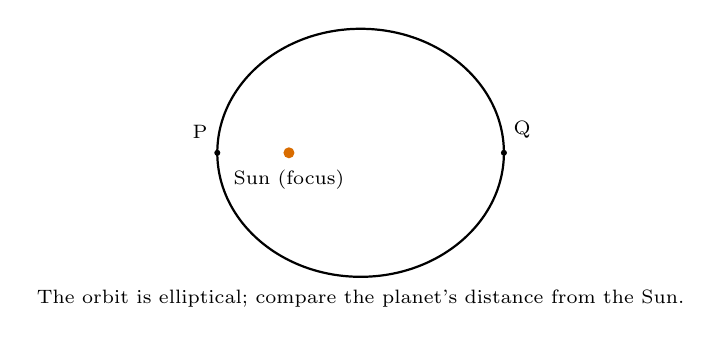
\begin{tikzpicture}[scale=0.70,font=\small]
  \draw[thick] (0,0) ellipse [x radius=2.6,y radius=2.25];
  \fill[orange!85!black] (-1.30,0) circle (0.10);
  \node[below] at (-1.30,-0.14) {\scriptsize Sun (focus)};
  \fill[black] (-2.60,0) circle (0.055);
  \fill[black] (2.60,0) circle (0.055);
  \node[above left] at (-2.60,0.08) {\scriptsize P};
  \node[above right] at (2.60,0.08) {\scriptsize Q};
  \node[align=center] at (0,-2.65)
    {\scriptsize The orbit is elliptical; compare the planet's distance from the Sun.};
\end{tikzpicture}
\end{center}

\vspace{0.4cm}

\textbf{A9.} The gravitational PE of a $1\ \text{kg}$
mass at Earth's surface (taking $\infty$ as zero) is
approximately ($R_E = 6.4\times10^6\ \text{m}$,
$g = 9.81\ \text{m\,s}^{-2}$):

\mcoption{A}{$-9.81\ \text{J}$}
\mcoption{B}{$-6.28\times10^7\ \text{J}$}
\mcoption{C}{$+6.28\times10^7\ \text{J}$}
\mcoption{D}{Zero}
\ansref{Ch8-A9}

\vspace{0.4cm}

\textbf{A10.} A geostationary satellite must be
placed:

\mcoption{A}{Above the poles}
\mcoption{B}{Above the equator with period 24 hours}
\mcoption{C}{At any altitude with speed matching
Earth's rotation}
\mcoption{D}{At $400\ \text{km}$ altitude}
\ansref{Ch8-A10}

\vspace{0.6cm}

\subsection*{Section B: Theory and Calculations}

\textbf{B1.} Two uniform spheres, each of mass
$M = 5.0\times10^3\ \text{kg}$ and radius
$0.50\ \text{m}$, are placed with their surfaces
touching.\\[4pt]
(a) Calculate the gravitational force between them.\\
(b) Compare this with the weight of one sphere
on Earth and comment.\\
(c) If the spheres are moved so their centres are
$4.0\ \text{m}$ apart, how does the force change?
Show using the inverse square law.
\hfill\ansref{Ch8-B1}

\vspace{0.4cm}

\textbf{B2.} A space probe is launched vertically
from Earth's surface.
($M_E = 5.97\times10^{24}\ \text{kg}$,
$R_E = 6.4\times10^6\ \text{m}$,
$G = 6.67\times10^{-11}\ \text{N\,m}^2\text{kg}^{-2}$)\\[4pt]
(a) Calculate the escape velocity from Earth.\\
(b) If the probe is launched at $8.0\ \text{km\,s}^{-1}$,
does it escape? Justify using energy.\\
(c) At what height above the surface is the
gravitational PE equal to half of its surface value
(i.e.\ where does $|E_p| = \frac{1}{2}|E_{p,surface}|$)?\\
(d) What is the probe's speed at that height if
launched at escape velocity?
\hfill\ansref{Ch8-B2}

\vspace{0.4cm}

\textbf{B3.} Jupiter has mass $1.90\times10^{27}\ \text{kg}$
and radius $7.15\times10^7\ \text{m}$.
Its moon Io orbits at $4.22\times10^8\ \text{m}$ from
Jupiter's centre.
($G = 6.67\times10^{-11}\ \text{N\,m}^2\text{kg}^{-2}$)\\[4pt]
(a) Calculate the gravitational field strength at
Jupiter's surface.\\
(b) Calculate the orbital speed of Io.\\
(c) Calculate the orbital period of Io in hours.\\
(d) Verify Kepler's Third Law using your results and
the data that Europa orbits at $6.71\times10^8\ \text{m}$
with period $85.2$ hours.
\hfill\ansref{Ch8-B3}

\vspace{0.4cm}

\textbf{B4.} Show that for a satellite in a circular
orbit at radius $r$ from Earth's centre:\\[4pt]
(a) The kinetic energy is $KE = GMm/(2r)$.\\
(b) The gravitational PE is $E_p = -GMm/r$.\\
(c) The total energy is $E_{total} = -GMm/(2r)$.\\
(d) The total energy is negative. Explain physically
why a satellite in orbit has negative total energy.\\
(e) Compare the total energy of a satellite at orbital
radius $r$ with one at $2r$. Which is easier to
reach from Earth, and why?
\hfill\ansref{Ch8-B4}

\vspace{0.4cm}

\textbf{B5.} (a) Using $g_s = GM_E/R_E^2$ and
$v_{esc} = \sqrt{2gR}$, show that the escape
velocity can be written as:
\[
  v_{esc} = R_E\sqrt{\frac{2g_s}{1}}
\]
(b) The temperature of a gas determines the average
speed of its molecules. Hydrogen molecules at room
temperature ($300\ \text{K}$) have an average speed
of about $1900\ \text{m\,s}^{-1}$.
Given that Earth's escape velocity is
$11\,200\ \text{m\,s}^{-1}$, explain why Earth retains
its nitrogen-oxygen atmosphere but loses hydrogen.\\
(c) The Moon's escape velocity is
$2370\ \text{m\,s}^{-1}$. Explain why the Moon
has no atmosphere at all.\\
(d) A student suggests that on a very hot planet
close to the Sun, liquid water could not exist on
the surface. Explain why in terms of escape velocity
and molecular speeds.
\hfill\ansref{Ch8-B5}

\end{exercisebox}

